\documentclass[table,dvipsnames]{beamer}
\mode<presentation>{
\usetheme{Madrid}
\setbeamercolor{title}{fg=Black,bg=Blue!15}
\setbeamercolor{frametitle}{fg=Black,bg=Blue!15}
\setbeamercolor{block title}{fg=Black,bg=Blue!15}
\setbeamercolor{block}{fg=Black,bg=Blue!10}
}

\usepackage{default}
\usepackage{graphicx}
\usepackage{booktabs}
\usepackage{xcolor}
\usepackage{multirow}

\title[Robot Vision]{Rancang Bangun \textit{Robot Vision} Untuk \textit{Object Finding} Menggunakan \textit{Color Tracking} pada perangkat RaspberryPi}
\author{}
\institute[Achmadi ITS]
{
Institut Teknologi Sepuluh November  \\
\vspace{10pt}
Oleh: \\
Achmadi 2410100085\\
\vspace{10pt}
Pembimbing:\\
Ir. Apriani K. MSc NIP: 195304041979012001
\medskip
\textit{}
}
\date{}

\begin{document}

\section{Judul}

\begin{frame}
\titlepage
\end{frame}

%\begin{frame}
%\frametitle{Overview}
%\tableofcontents
%\end{frame}

\section{Pendahuluan}

\subsection{Latar Belakang}

\begin{frame}
\frametitle{Latar Belakang}
\framesubtitle{Robot Membantu Manusia}
\begin{center}
 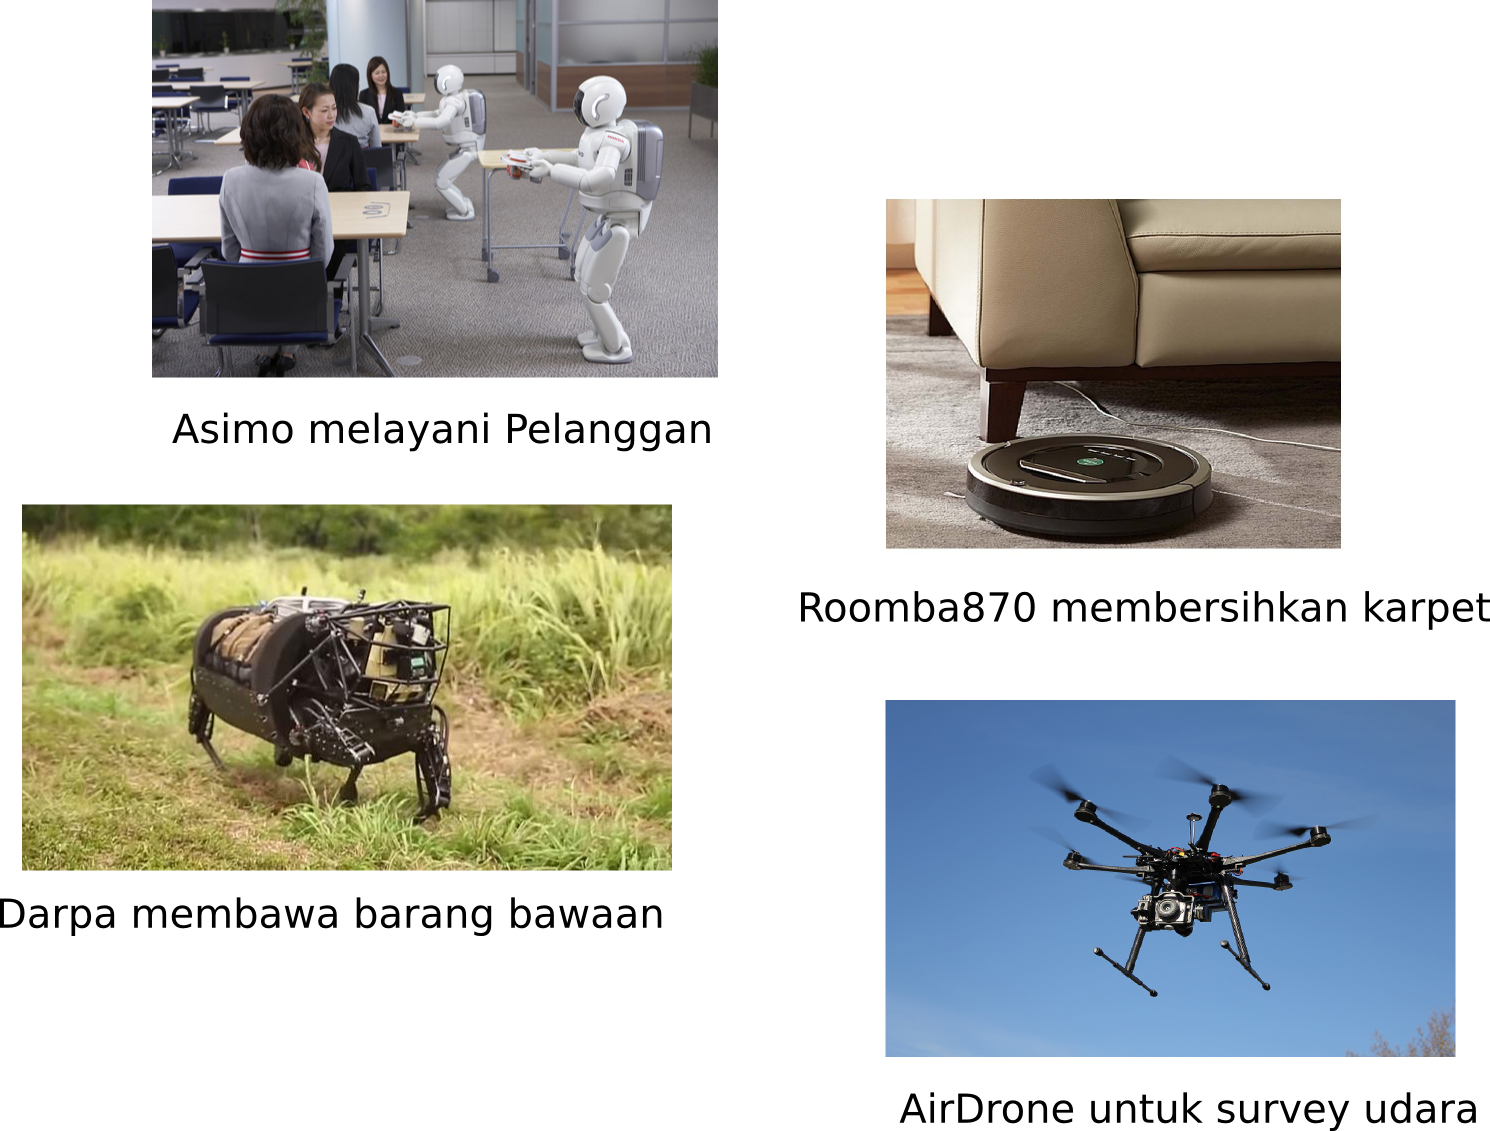
\includegraphics[width=250pt]{./latar_belakang/robot_membantu_manusia/robot_melayani}
\end{center}
\end{frame}

\begin{frame}
\frametitle{Latar Belakang}
\framesubtitle{Sensor Robot}
\begin{center}
 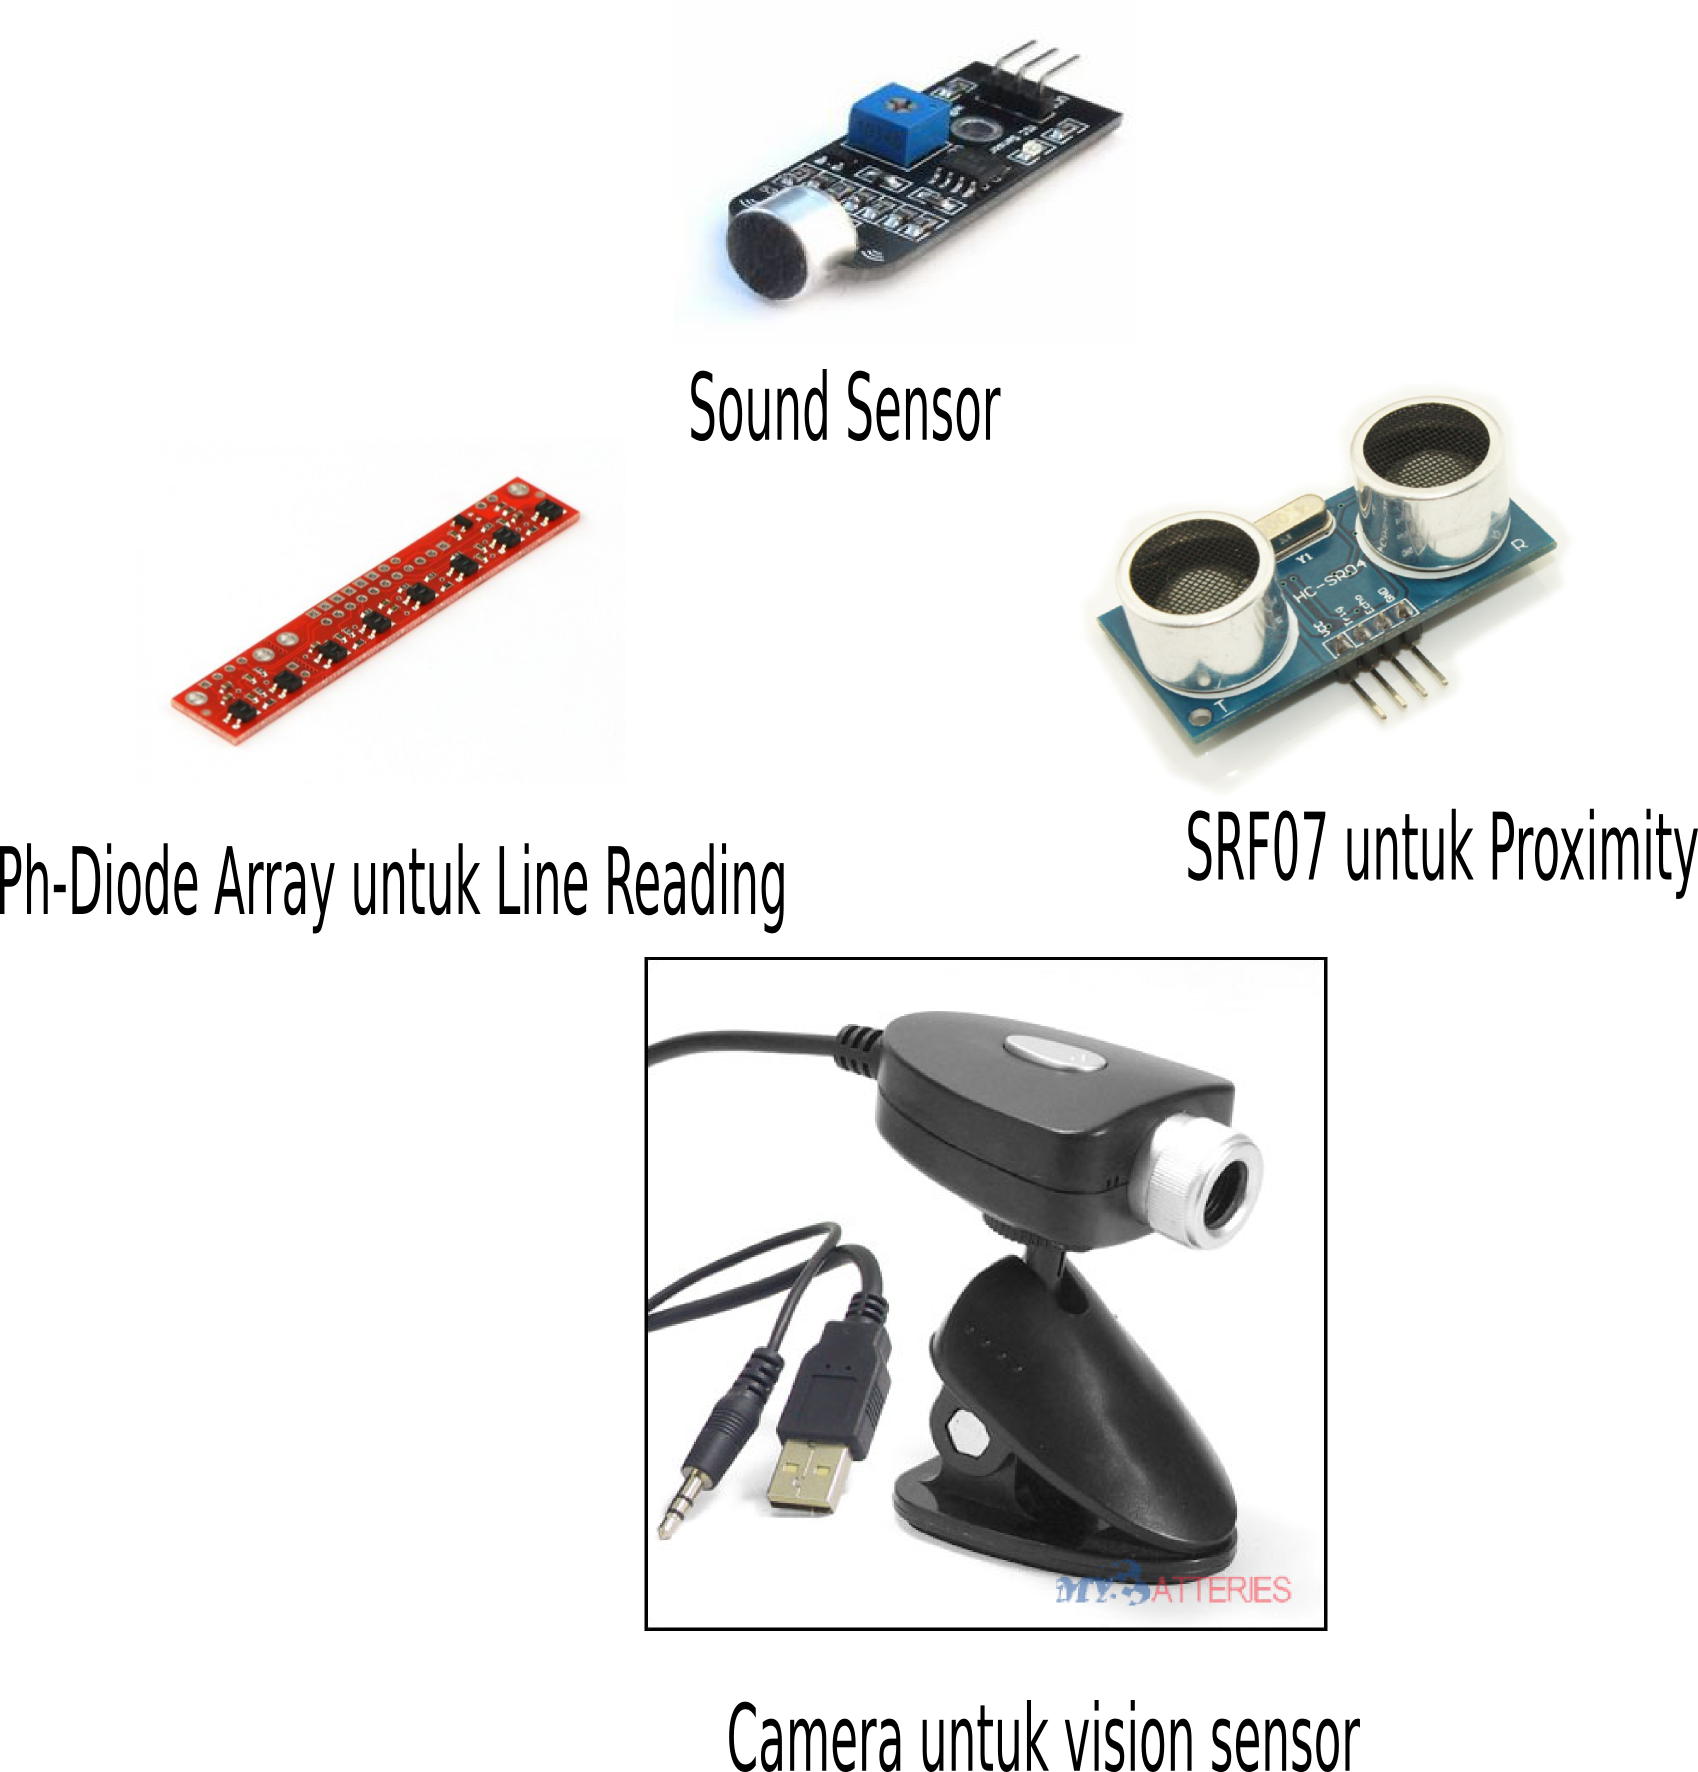
\includegraphics[width=200pt]{./latar_belakang/sensor_robot/sensor}
\end{center}
\end{frame}

\begin{frame}
\frametitle{Latar Belakang}
\framesubtitle{Robot Vision}
\begin{block}{\cite{why_vision}}
Dengan ketersediaannya yang luas, konten informasi tinggi, dan kesesuaian untuk lingkungan manusia serta harga yang murah dari kamera warna, sistem vision menjadi cocok untuk banyak platform robot.
\end{block}
\end{frame}

\begin{frame}
\frametitle{Latar Belakang}
\framesubtitle{Contoh Vision: Asimo}
\begin{center}
 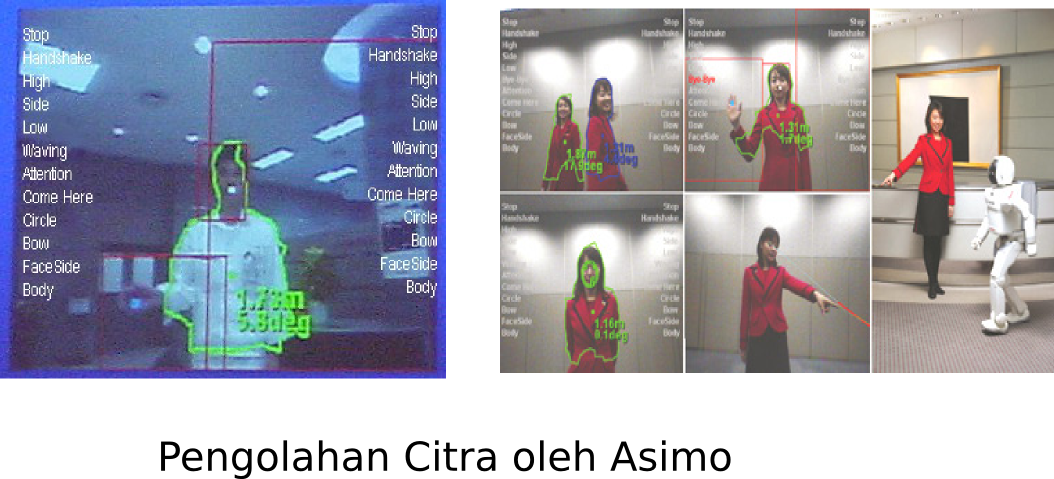
\includegraphics[width=200pt]{./latar_belakang/asimo_vision/asimo_vision}
\end{center}
\begin{block}{\cite{asimo_cpu}}
Jenis Kamera : CCD\\
Processor : 20 Unit Honda Propietary CPU\\
Harga : \$2.500.000\\
\end{block}
\end{frame}

\begin{frame}
\frametitle{Latar Belakang}
\framesubtitle{Single Board Computer Raspberry Pi}
\begin{center}
 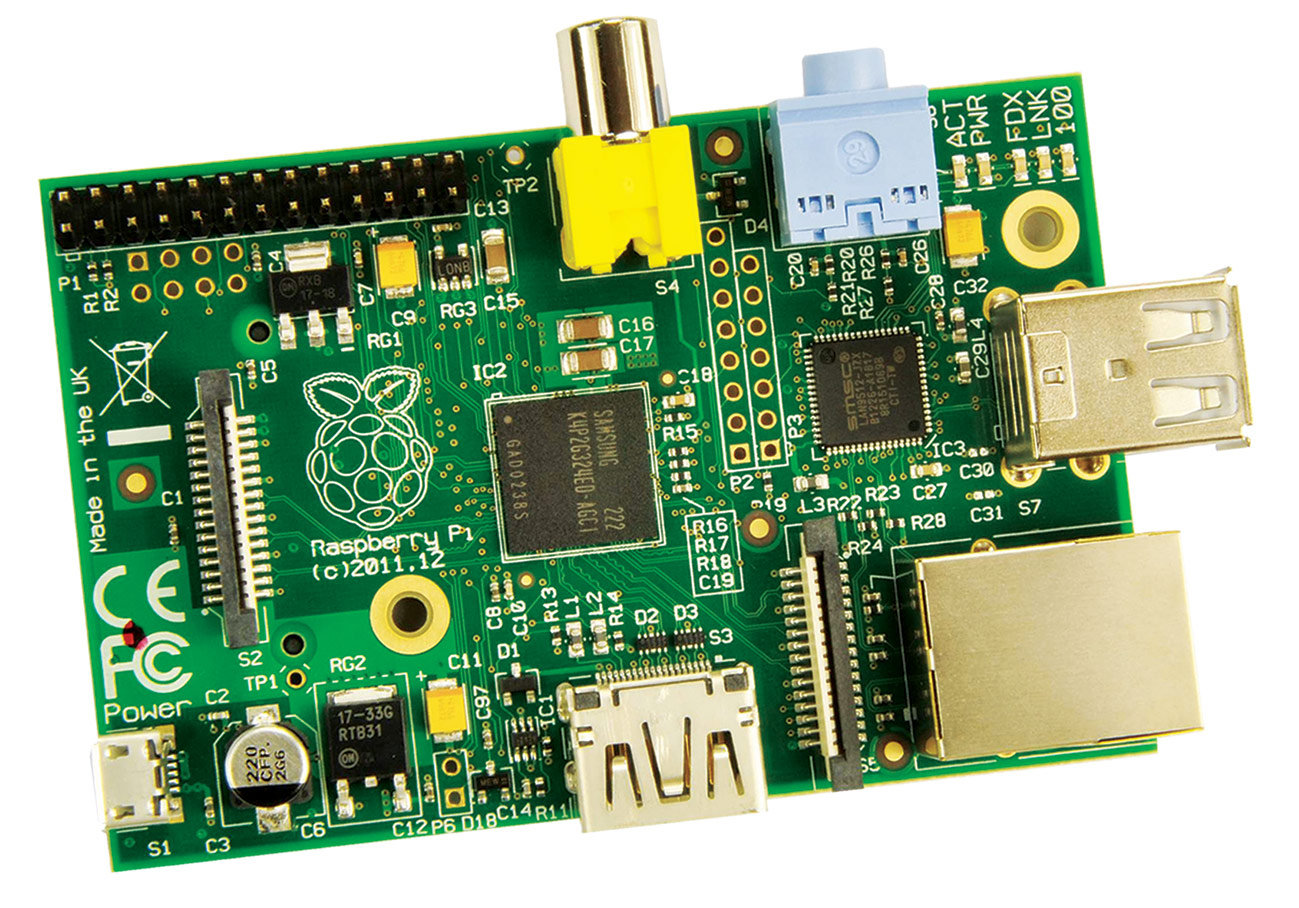
\includegraphics[width=150pt]{./latar_belakang/raspi/raspi}
\end{center}
\begin{block}{Single-Board Computer RaspberryPi B (\$60)}
CPU : 700 MHz\\
RAM : 512 MB\\
USB	: 2x USB 2.0\\
HMI : HDMI\\
\end{block}
\end{frame}

\subsection{Rumusan Masalah}

\begin{frame}
\frametitle{Rumusan Masalah}
\begin{block}{}
Bagaimana merancang bangun robot vision berbasis color tracking menggunakan OpenCV pada perangkat RaspberryPi.
\end{block}
\end{frame}

\subsection{Batasan Masalah}

\begin{frame}
\frametitle{Batasan Masalah}
\begin{block}{}
Posisi objek terhadap robot telah ditentukan.
\end{block}
\begin{block}{}
Objek yang akan diolah telah ditentukan ukuran dan warnanya.
\end{block}
\begin{block}{}
Robot bekerja pada tingkat pencahayaan yang telah diatur.
\end{block}
\end{frame}

%\begin{frame}
%\frametitle{Overview}
%\tableofcontents
%\end{frame}

\section{Teori Penunjang}

\subsection{Robot Vision}

\begin{frame}
\frametitle{Robot Vision}
\begin{block}{\cite{robot_vis}}
 Robot Vision adalah mesin automatis atau semi-automatis yang mampu memperoleh informasi melalui proses akuisisi dan pemrosesan citra.
\end{block}
\end{frame}


\subsection{Object Finding}

\begin{frame}
\frametitle{Menemukan suatu objek (Object Finding)}
\begin{block}{}
Robot mampu mendapatkan posisi objek terhadap dirinya berdasarkan pengolahan citra yang didapatkan oleh kamera yang ada pada robot.
\end{block}
\begin{block}{}
Robot mampu mendekati objek berdasarkan informasi yang diperoleh dari proses penentuan posisi sebelumnya.
\end{block}
\end{frame}

\subsection{Mode Warna HSV}

\begin{frame}
\frametitle{Mode Warna HSV}
\begin{block}{}
Mode Warna yang mengkarakteristikan warna dalam 3 variabel, yaitu Hue, Saturation, dan Value
\end{block}
\begin{block}{}
Hue adalah nilai warna dalam satuan sudut.
Hue di plot dalam diagram berbentuk lingkaran dengan warna Red, Green, dan Blue terpisah dalam sudut 120 derajat.
Warna lainnya merupakan tingkat campuran dari ketiga warna tersebut.
\end{block}
\begin{block}{}
Saturation adalah nilai tingkat suatu warna terhadap warna Hitam.\\
Tingkat Pencahayaan dapat mempengaruhi nilai Saturation.
\end{block}
\begin{block}{}
Value adalah nilai tingkat suatu warna terhadap warna Putih.\\
Tingkat Pencahayaan dapat mempengaruhi nilai Saturation.
\end{block}
\end{frame}

\begin{frame}
\frametitle{Mode Warna HSV}
\begin{block}{Diagram HSV}
\begin{center}
 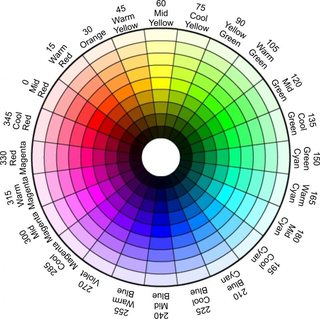
\includegraphics[width=200pt]{./tinjauan_teori/hsv/HSV}
\end{center}
\end{block}
\end{frame}

\begin{frame}
\frametitle{Mode Warna HSV}
\begin{block}{Konversi RGB ke HSV}
Kamera menghasilkan gambar dalam mode RGB maka perlu dikonversi ke HSV sebelum proses lebih lanjut.
\begin{equation}
  V = max(R,G,B)
\end{equation}
\begin{equation}
  S =  
  \begin{cases}
      \frac{V-min(R,G,B)}{V},& \text{jika } V\neq 0\\
      0,              & \text{jika } V = 0\\
  \end{cases}
\end{equation}
\begin{equation}
  H =  
  \begin{cases}
      \frac{60(G-B)}{(V-min(R,G,B))},& \text{jika } V = R\\
      120 + \frac{60(B-R)}{(V-min(R,G,B))},& \text{jika } V = G\\
      240 + \frac{60(R-G)}{(V-min(R,G,B))},& \text{jika } V = B\\
  \end{cases}
\end{equation}
\end{block}
\end{frame}

\subsection{Thresholding}

\begin{frame}
\frametitle{Thresholding}
\begin{block}{}
Thresholding adalah proses menyeleksi pixel berdasarkan range nilai HSV yang telah ditentukan.
\end{block}
\begin{block}{}
Untuk pixel (8bit) yang sesuai jangkauan maka nilainya dikonversi ke 255 (putih).
Jika tidak sebaliknya maka nilainya dikonversi ke 0 (hitam).
\begin{equation}
  P(i,j) =  
  \begin{cases}
      255,& H_{min} \leq H\leq H_{max} \land S_{min} \leq S\leq S_{max} \land V_{min} \leq V\leq V_{max}\\
      0,              & \text{ selainnya } \\
  \end{cases}
\end{equation}
\end{block}
\begin{block}{}
Konversi ke binary image.
\begin{equation}
  B(i,j) =  
  \begin{cases}
      1,& P(i,j)=255\\
      0,& P(i,j)=0 \\
  \end{cases}
\end{equation}
\end{block}
\end{frame}

\begin{frame}
\frametitle{Jangkauan Thresholding}
\begin{block}{Jangkauan HSV untuk warna Merah}
\begin{equation}
160 \leq H\leq 179
\end{equation}
\begin{equation}
171 \leq S\leq 255
\end{equation}
\begin{equation}
120 \leq V\leq 255
\end{equation}
\end{block}
\begin{block}{Contoh hasil Thresholding}
\begin{center}
 \includegraphics[width=100pt]{../../proposal/imgori}
 
\includegraphics[width=100pt]{../../proposal/imgthresh}
\end{center}
\end{block}
\end{frame}

\subsection{Titik Pusat}

\begin{frame}
\frametitle{Titik Pusat}
\begin{block}{}
Titik Pusat (Centroid) adalah titik yang menjadi pusat luasan dari total luas pixel.
Titik ini identik dengan pusat massa untuk benda 2D.
\begin{equation}
\overline{x}=\frac{x1*m1 + x2*m2 + x3*m3 +...}{m1 + m2 + m3 +...}
\end{equation}
\begin{equation}
\overline{y}=\frac{y1*n1 + y2*n2 + y3*n3 +...}{n1 + n2 + n3 +...}
\end{equation}
\end{block}
\end{frame}

\subsection{OpenCV}

\begin{frame}
\frametitle{OpenCV}
\begin{block}{}
OpenCV (Open Computer Vision) adalah pustaka pemrograman untuk pengolahan citra yang bersifat opensource.
\end{block}
\begin{block}{}
OpenCV mendukung bahasa pemrograman C, C++, dan Python.
\end{block}
\begin{block}{}
OpenCV menyediakan fungsi-fungsi pengolahan citra yang lengkap mulai dari perhitungan histogram hingga algoritma Haar-Cascade untuk deteksi wajah.
\end{block}
\begin{block}{}
OpenCV dapat digunakan sebagai pengganti Matlab untuk proses pengolahan citra yang mengharuskan program ditulis dalam C atau C++.
\end{block}
\end{frame}

\subsection{Raspbian}

\begin{frame}
\frametitle{Raspbian}
\begin{block}{}
Raspbian adalah Operating System berbasis Debian yang dijalankan di platform RaspberryPi.
\end{block}
\begin{block}{}
Raspbian menggunakan kernel Linux untuk arsitektur armhf.
\end{block}
\begin{block}{}
Melalui Raspbian ini nantinya menjalankan OpenCV untuk pengolahan citra dan komunikasi serial untuk mengontrol robot.
\end{block}
\begin{block}{}
Lumbung Software (Repository) dari Raspbian telah menyediakan binary siap pakai sehingga memudahkan instalasi.
\end{block}
\end{frame}

\subsection{Rancangan Robot}

\begin{frame}
 \frametitle{Rancangan Bagian Robot}
 \begin{center}
 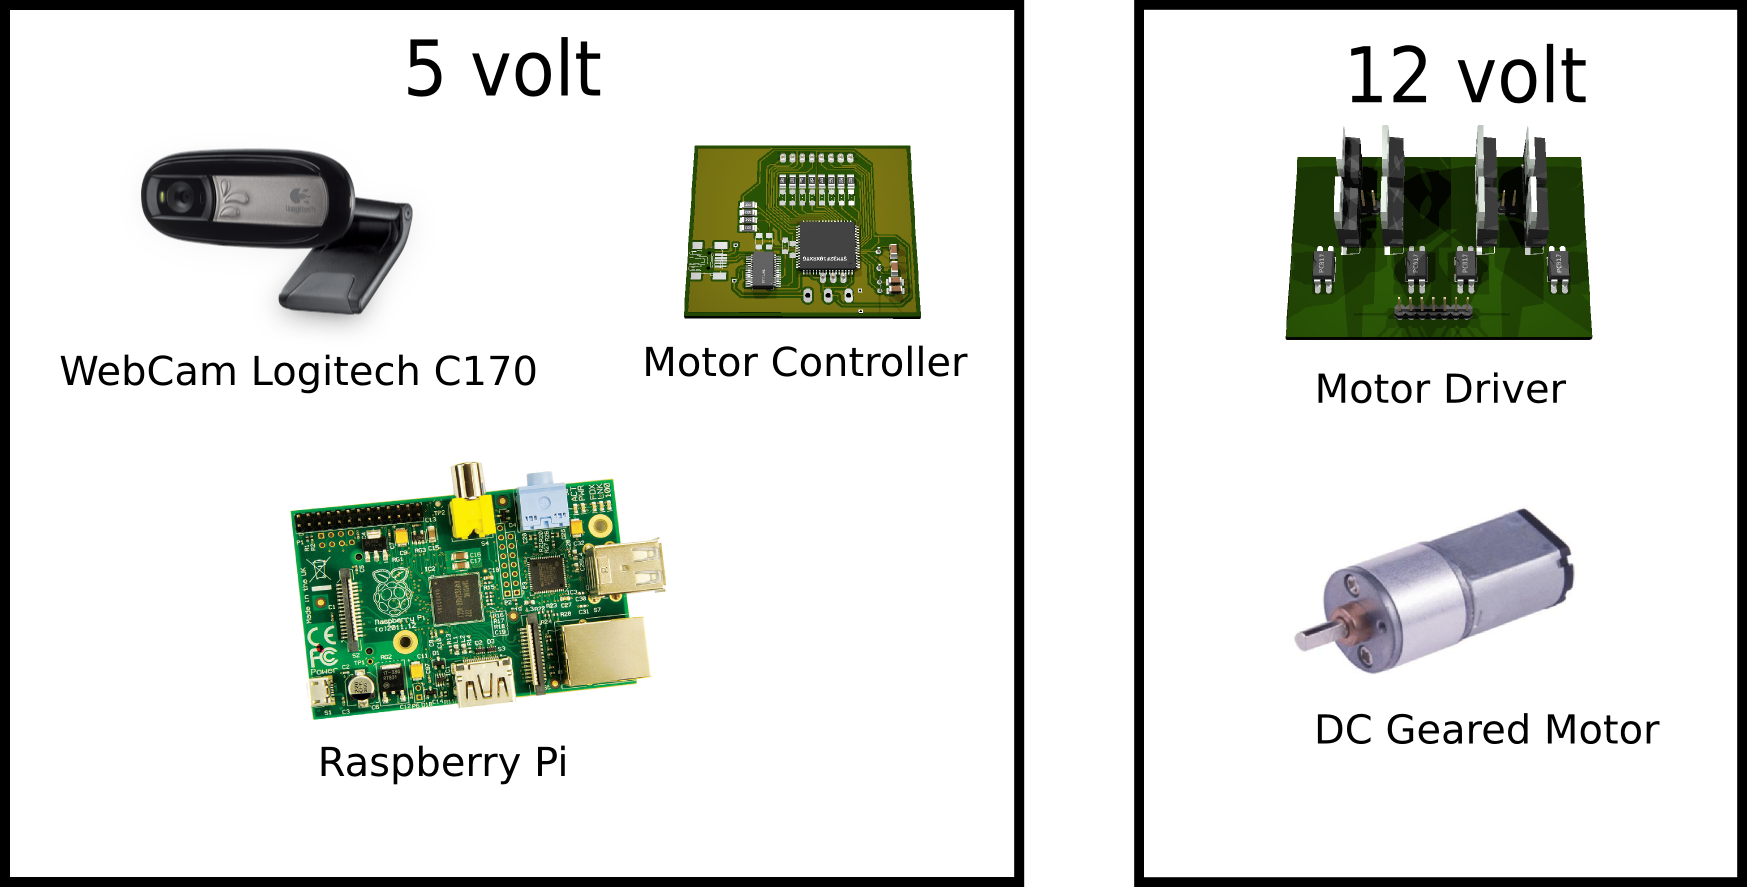
\includegraphics[width=300pt]{./bagian_robot/parts.png}
\end{center}
\end{frame}

\begin{frame}
\frametitle{Rancangan Flow Chart Robot}
% edit ke non-standard flowchart
% tambahkan simbol komponen
\begin{center}
 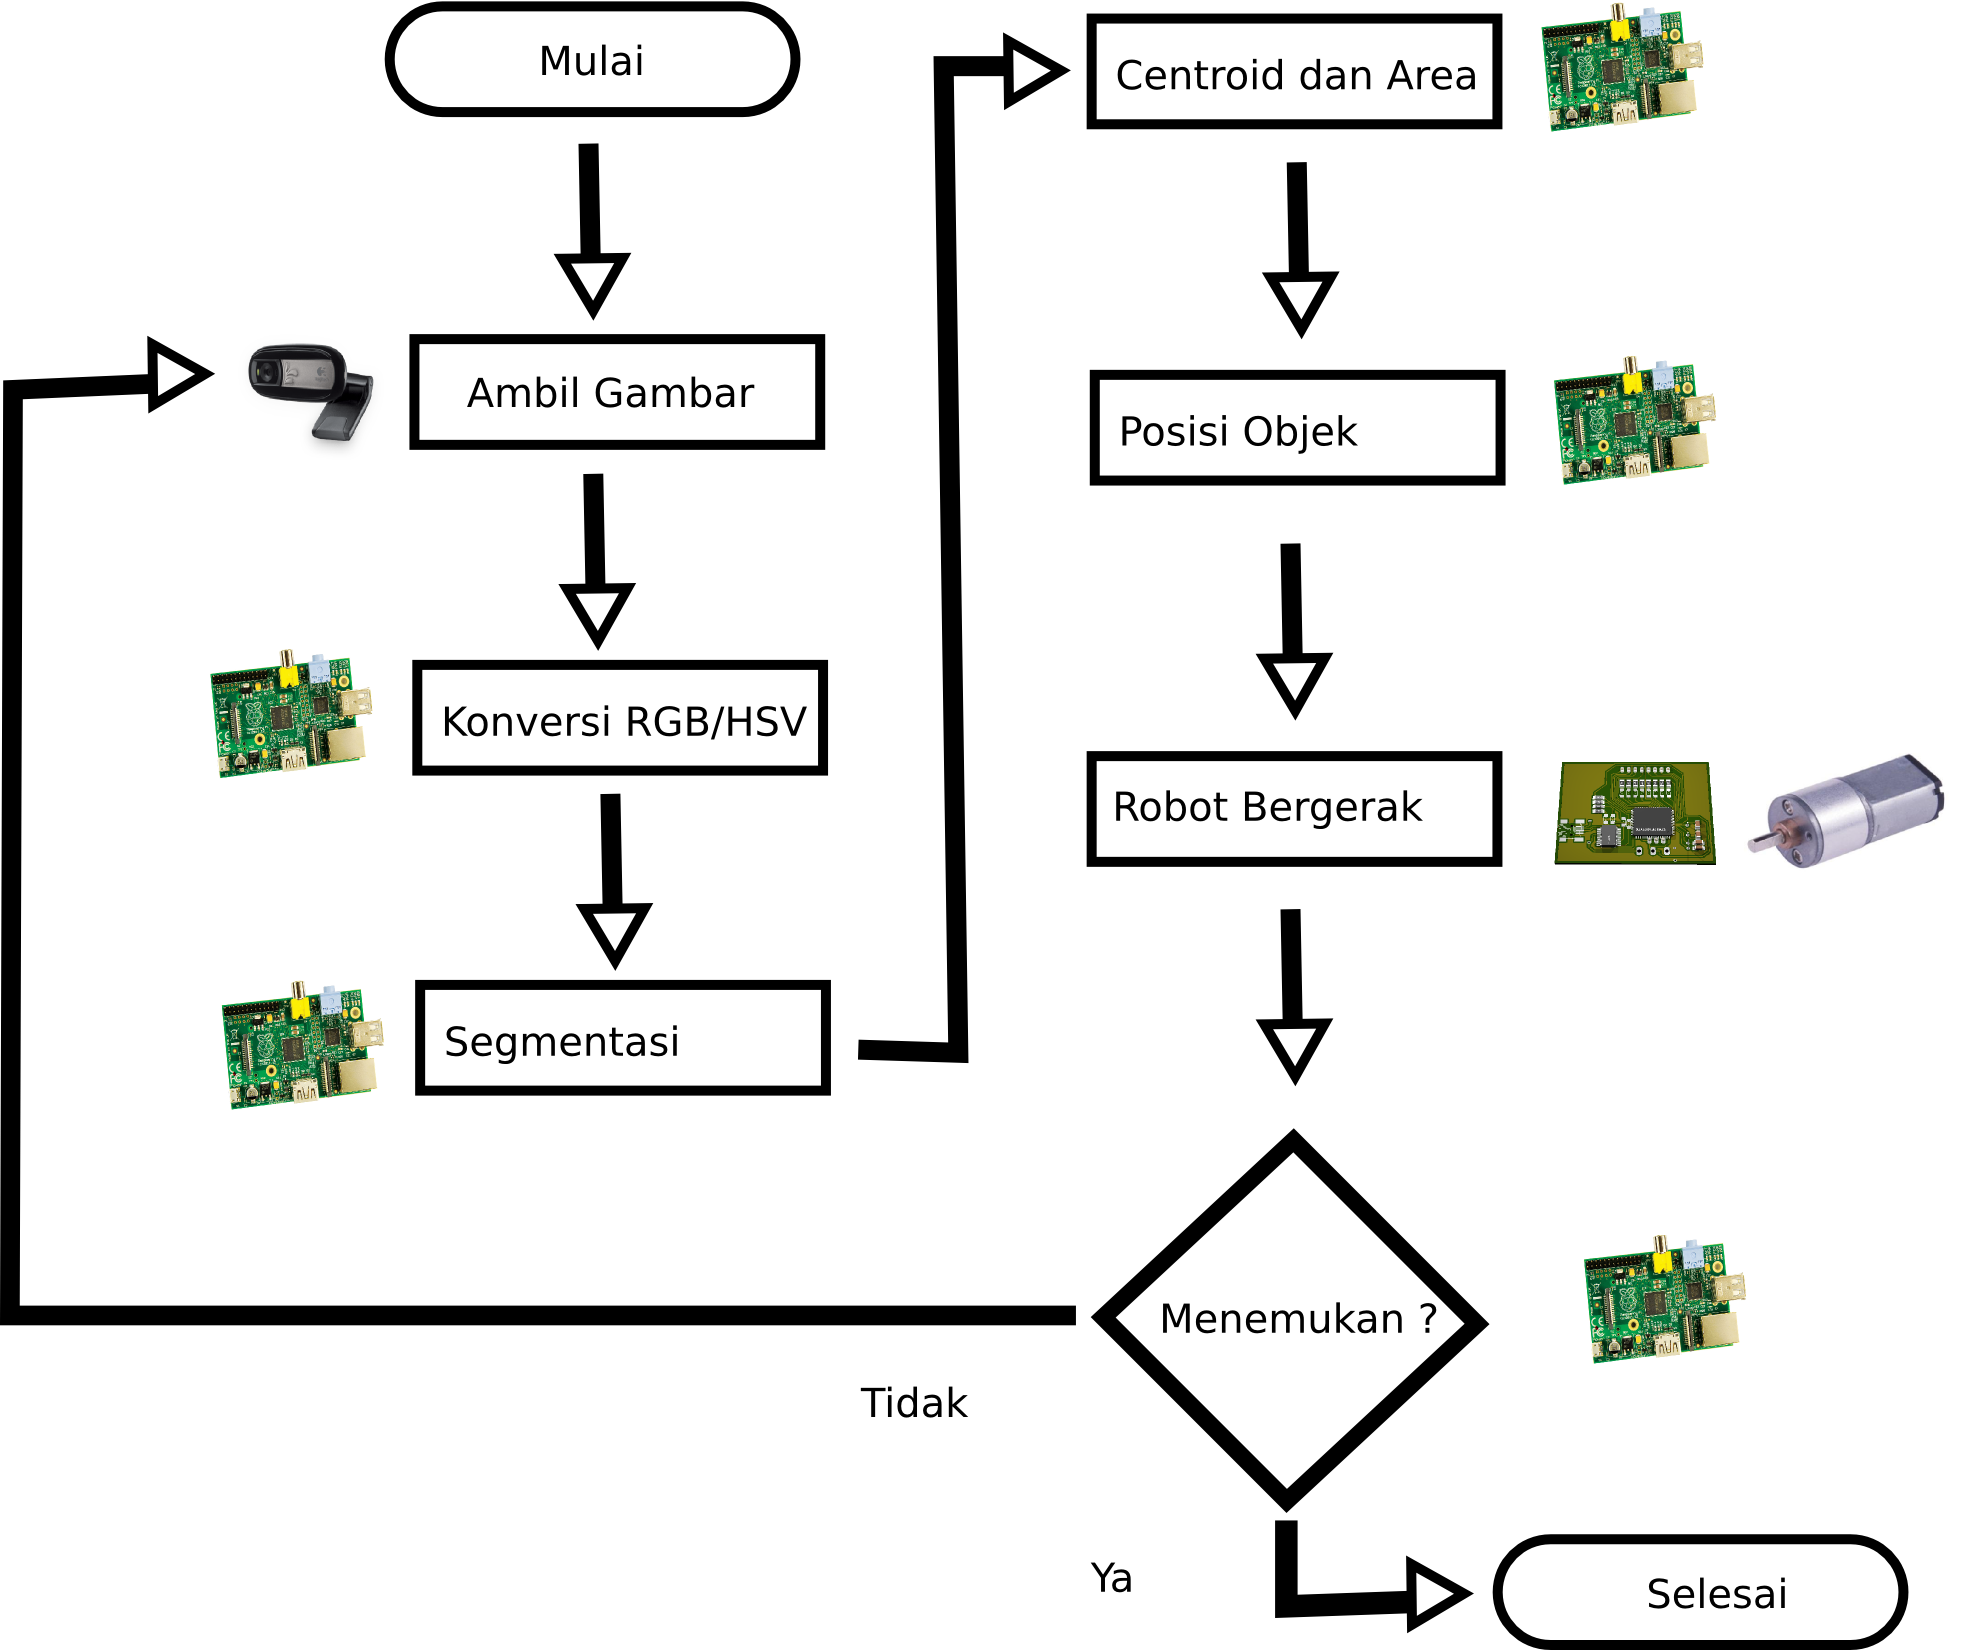
\includegraphics[width=250pt]{./proses_robot/process}
\end{center}
\end{frame}

%\begin{frame}
%\frametitle{Overview}
%\tableofcontents
%\end{frame}

\section{Metode Penelitian}

\begin{frame}
\frametitle{Flow Chart Pengerjaan}
% edit ke non-standard flowchart
\begin{center}
 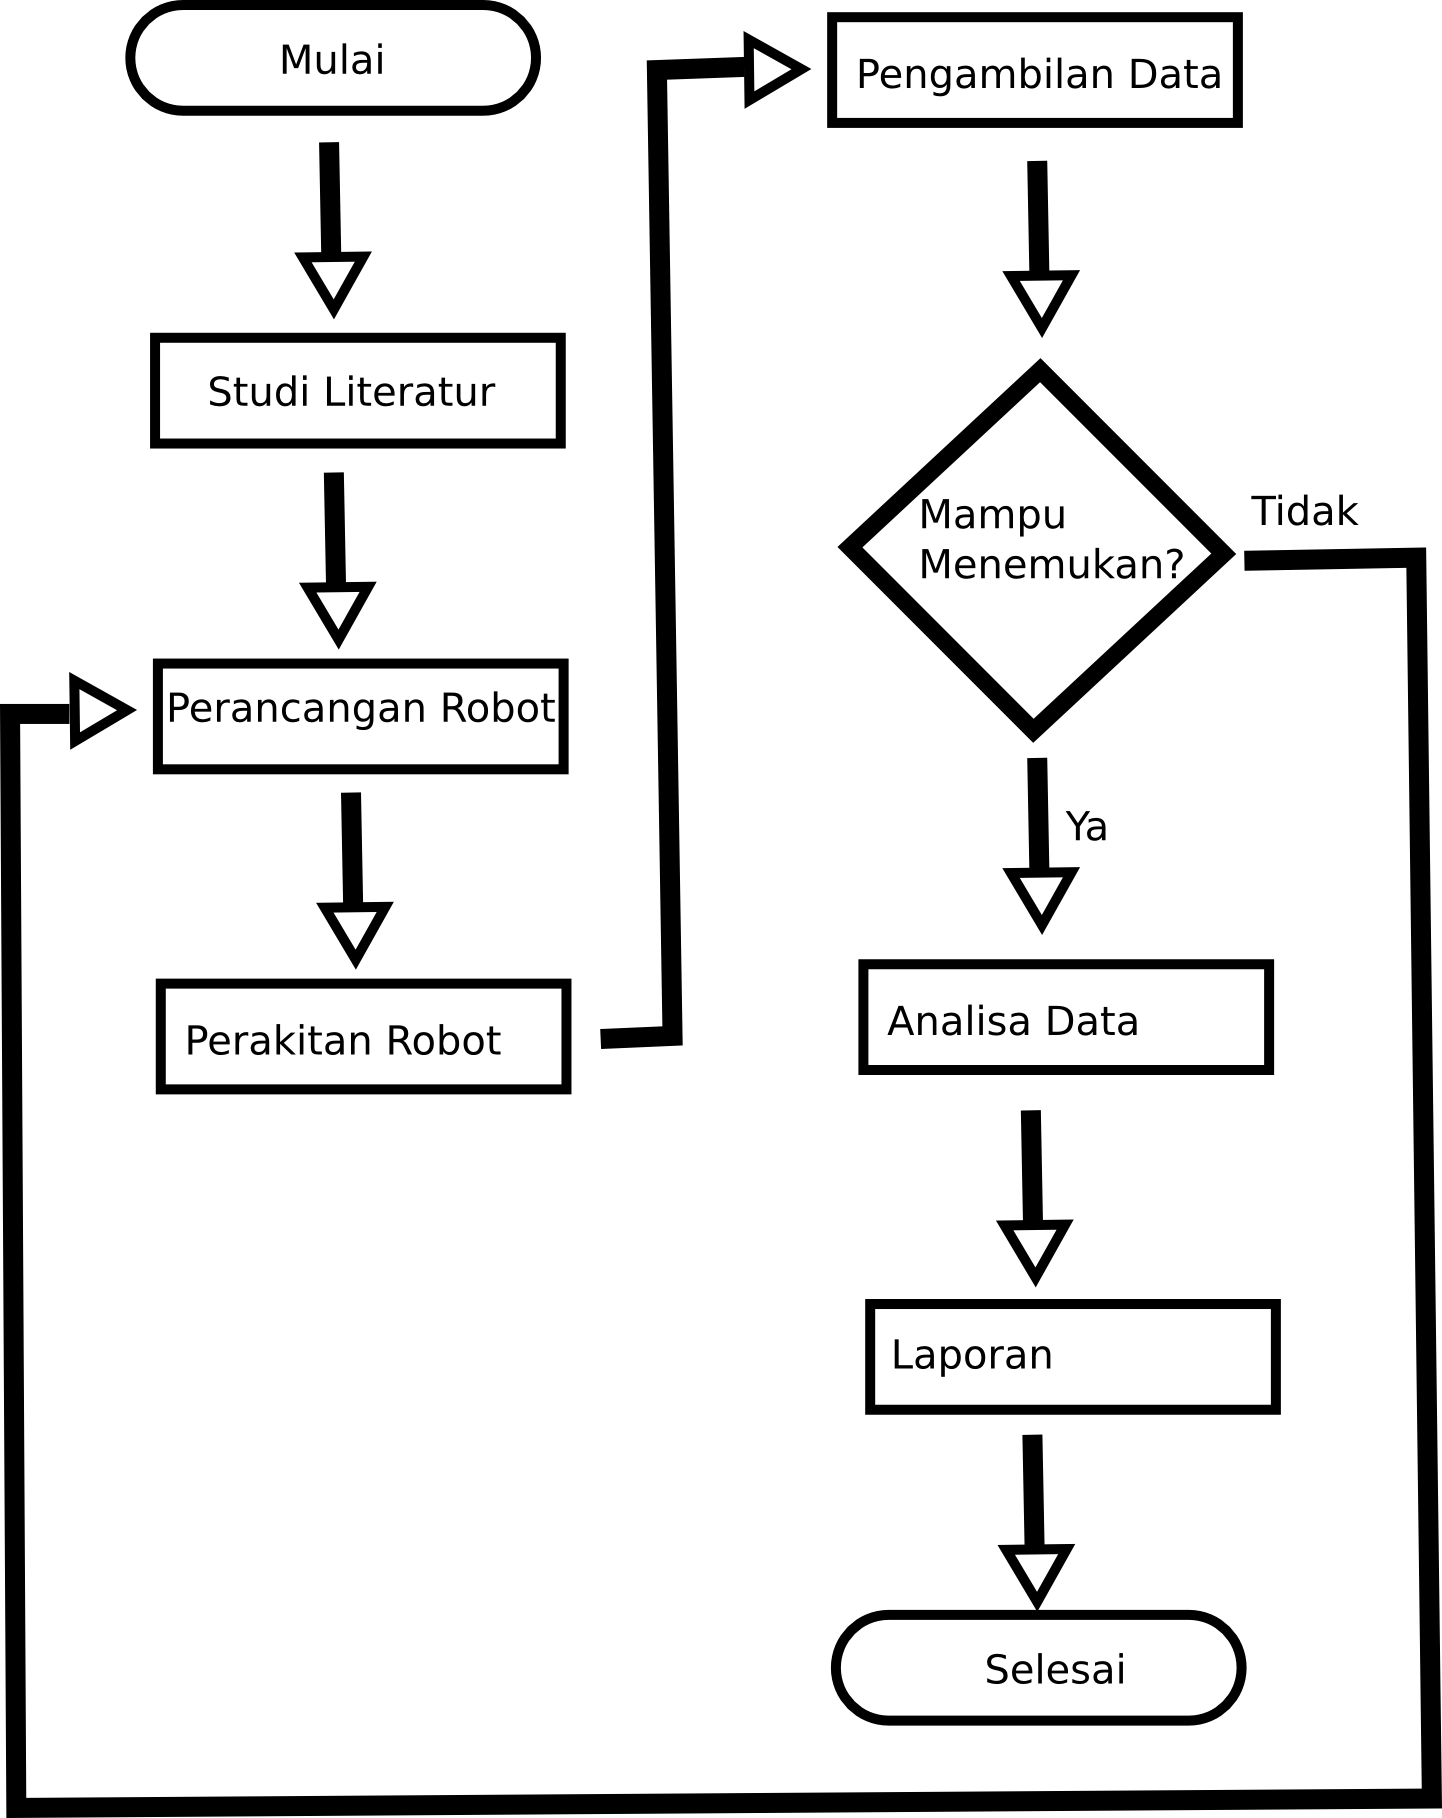
\includegraphics[width=150pt]{./pengerjaan/work}
\end{center}
\end{frame}

%\section{Jadwal Pengerjaan}
%
%\begin{frame}
%\frametitle{Jadwal Pengerjaan}
%\begin{table}
% \begin{tabular}{ |l|l|l|l|l|l| }
%   \hline
%   No & Kegiatan & \multicolumn{3}{|c|}{Bulan} \\
%   \hline
%     &  & Oktober & November & Desember \\
%   \hline
%   1 & Studi literatur & \cellcolor{blue} & \cellcolor{blue} & \\
%   \hline
%   2 & Perancangan dan Pembuatan & \cellcolor{blue} & \cellcolor{blue} & \\
%   \hline
%   3 & Pengambilan Data & & \cellcolor{blue} & \cellcolor{blue} \\
%   \hline
%   4 & Analisa Data & & & \cellcolor{blue} \\
%   \hline
%   5 & Penulisan Laporan & & \cellcolor{blue} & \cellcolor{blue} \\
%  \hline
%\end{tabular}
%\end{table}
%\end{frame}

\section{Daftar Pustaka}
% 
\begin{frame}
\frametitle{Daftar Pustaka}
\footnotesize{
\begin{thebibliography}{99}
\bibitem[Budiharto,2012]{robot_vis} Widodo Budiharto, Djoko Purwanto \textit{Robot Vision} 2012
\bibitem[Brett, 2010]{why_vision} Brett Browning, Manuela Veloso \textit{Real-Time, Adaptive Color-based Robot Vision} 2010
\bibitem[Honda, 2007]{asimo_cpu} Honda Public Division \textit{Asimo Technical Information} 2007
\bibitem{robot_vision} Aleš Ude \textit{Robot Vision} 2010
\bibitem{ccd} Andor Team \textit{Digital Camera Fundamentals} 2012
\bibitem{robot_function} Chao, Fei \textit{A developmental approach to robotic pointing via human–robot interaction} 2014
\bibitem{raspi} Upton, Eben \textit{RaspberryPi User Guide} 2012
\bibitem{opencv_intro} OpenCV Team \textit{The OpenCV Reference Manual} 2014
\bibitem{hsv} Phillips, Dwyne \textit{Image Processing in C} 2000
\bibitem{improc1} Zhou, Huiyu \textit{Digital Image Processing Part I} 2010
\end{thebibliography}
}
\end{frame}


\begin{frame}
\Huge{\centerline{Mator Sakalangkong}}
\end{frame}

% \section{Pencapaian terkini}
% 
% \begin{frame}
% \frametitle{Pencapaian terkini}
% \begin{block}{Hardware}
% Robot telah dirakit dan mampu bergerak sesuai perintah yang dikirim melalui komunikasi serial UART.
% \end{block}
% \begin{block}{Software}
% Robot telah dapat:
% \begin{itemize}
% \item Mengambil Citra dari WebCamera melalui jalur USB
% \item Mengkonversi gambar ke HSV
% \item Men-Treshold gambar sesuai jangkauan yang telah diatur
% \end{itemize}
% \end{block}
% \begin{block}{}
% VIDEO
% \end{block}
% \end{frame}
% 
% \begin{frame}
% \frametitle{Hasil Rakitan}
% \begin{center}
%  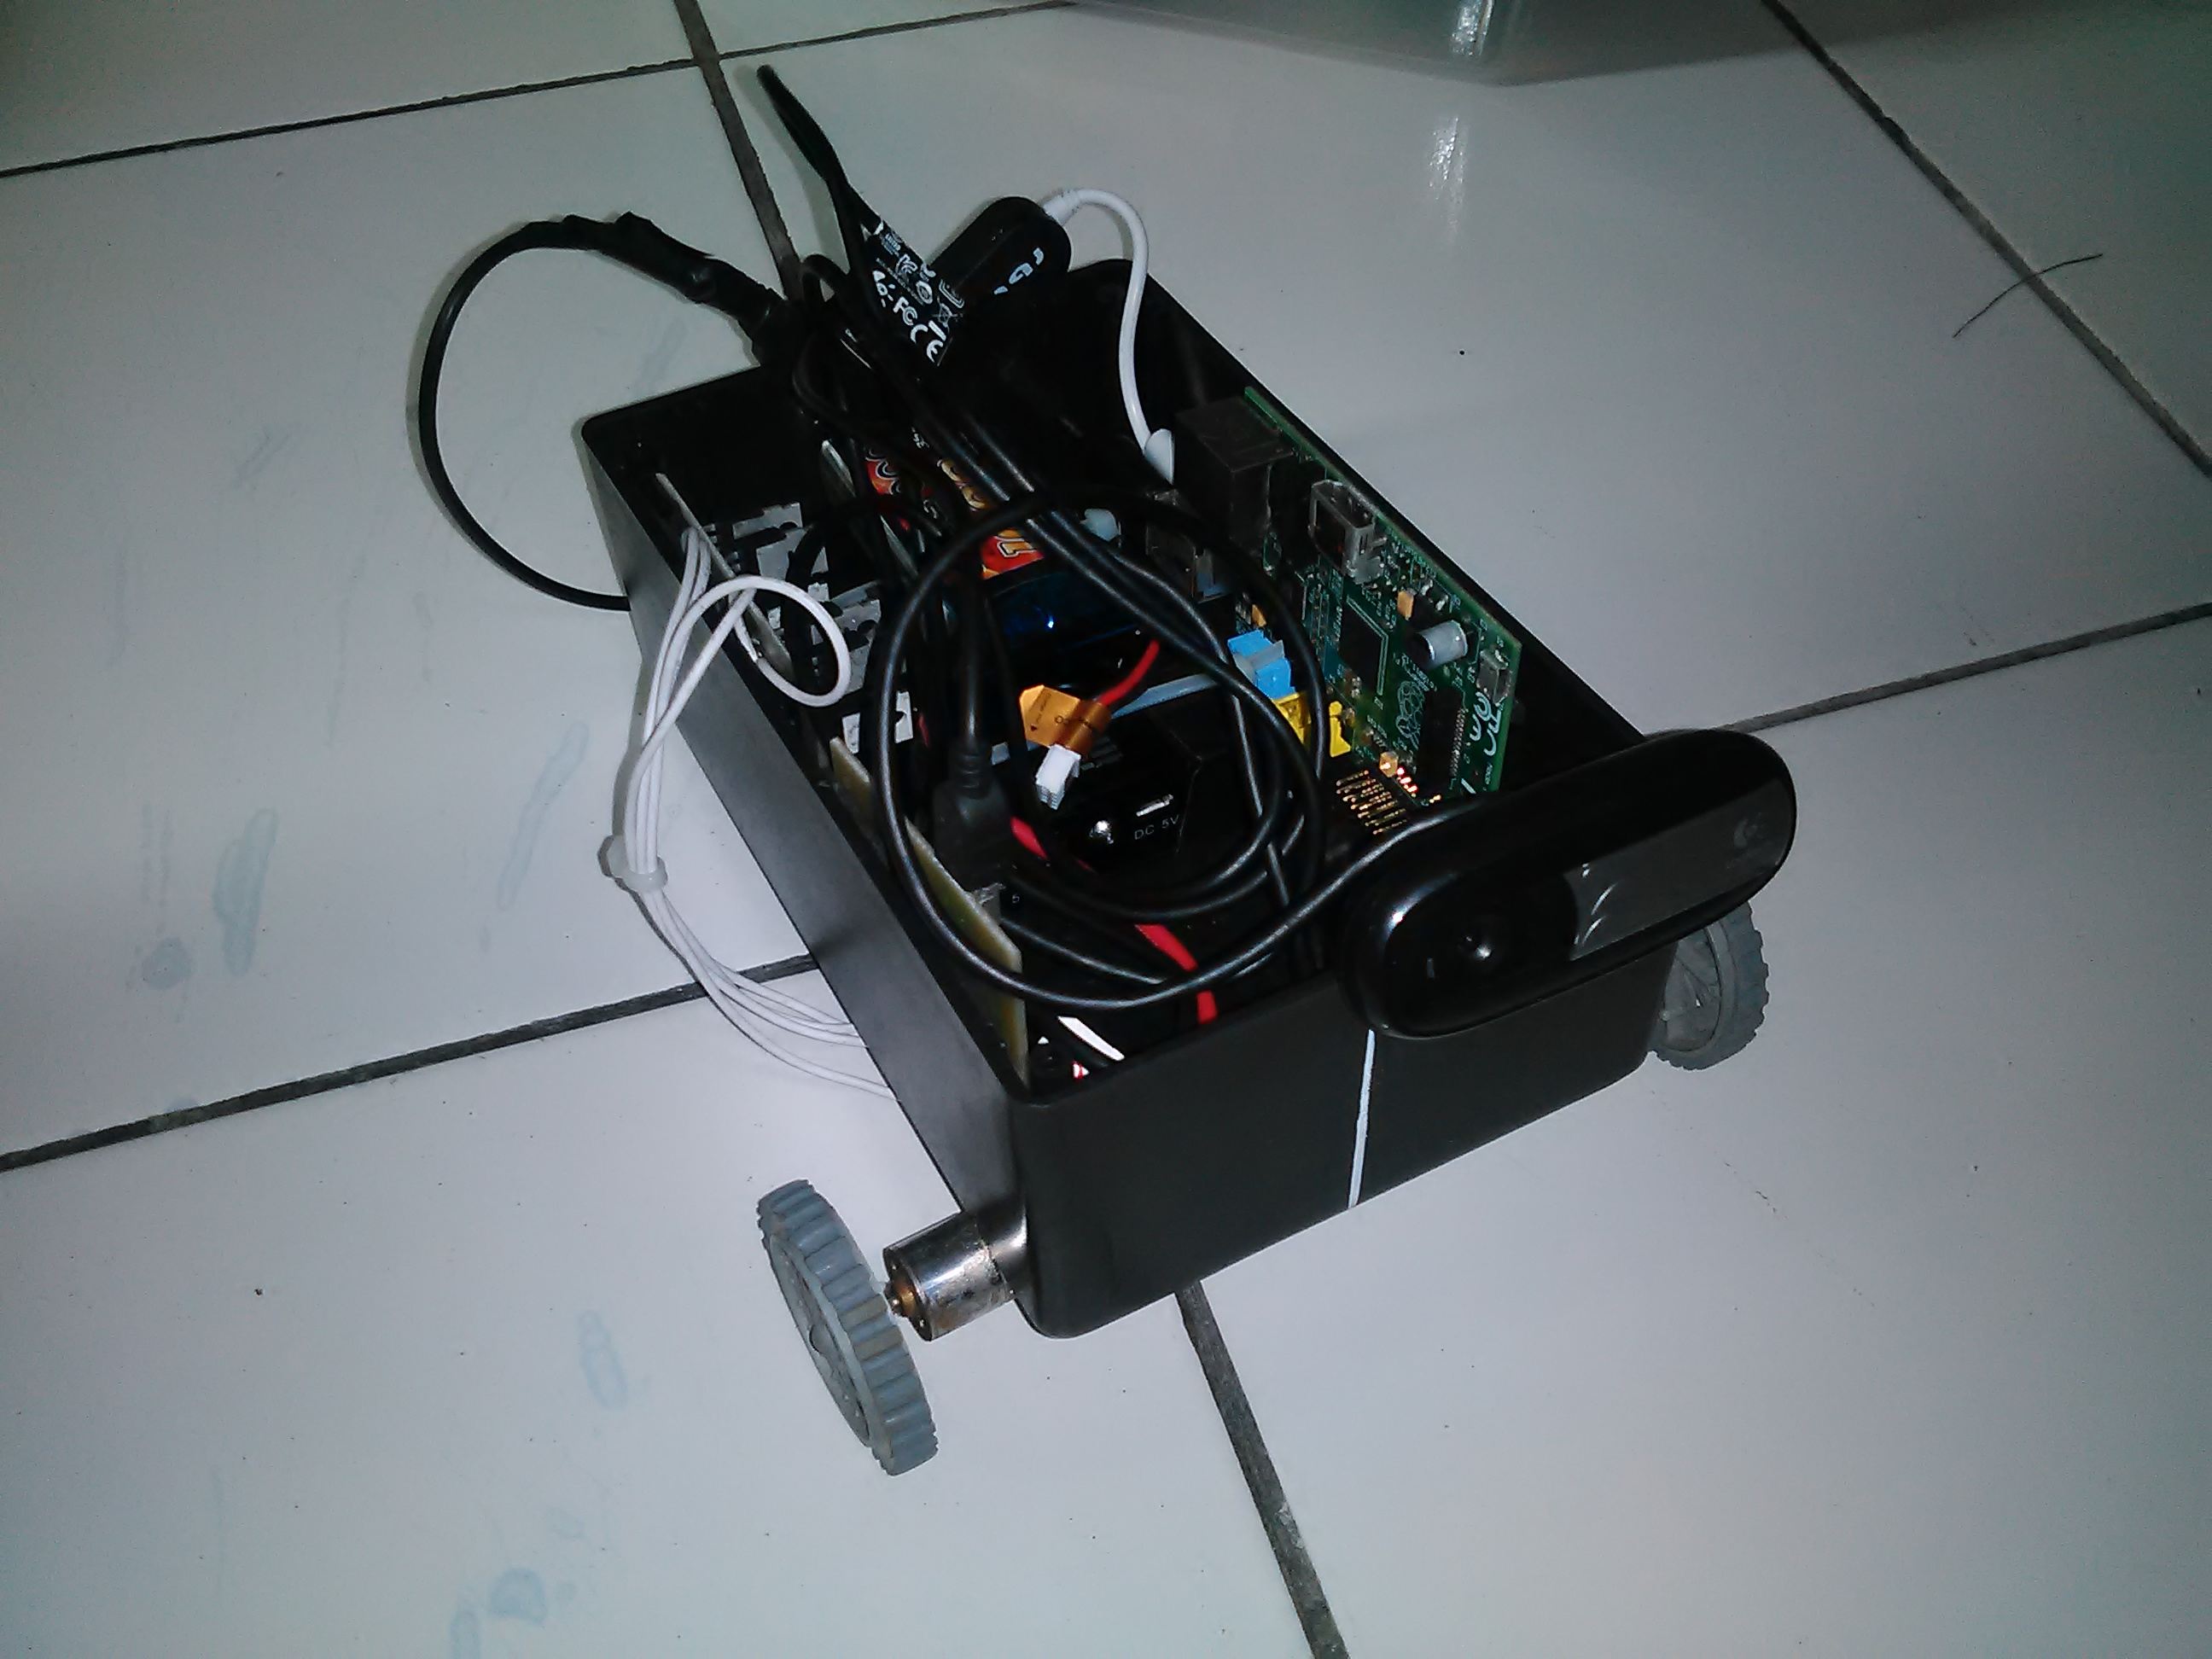
\includegraphics[width=200pt]{./progress/builded}
% \end{center}
% \end{frame}
% 
% \begin{frame}
% \frametitle{Detail Bagian}
% \begin{center}
%  
\includegraphics[width=250pt]{./progress/detail}
% \end{center}
% \end{frame}
% 
% \begin{frame}
% \frametitle{Flow Chart Robot}
% \begin{center}
%  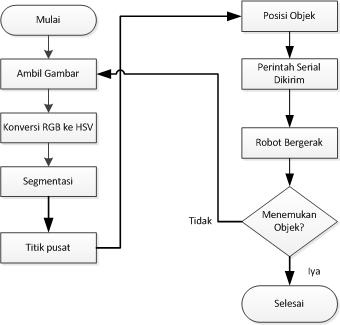
\includegraphics[width=200pt]{./progress/flowprogress}
% \end{center}
% \end{frame}

% \begin{frame}
% \frametitle{Jangkauan Thresholding}
% 
% \begin{block}{Jangkauan HSV untuk warna Merah}
% \begin{equation}
% 160 \leq H\leq 179
% \end{equation}
% \begin{equation}
% 171 \leq S\leq 255
% \end{equation}
% \begin{equation}
% 120 \leq V\leq 255
% \end{equation}
% \end{block}
% 
% \begin{block}{Contoh hasil Thresholding}
% \begin{center}
%  \includegraphics[width=100pt]{./progress/imgori}
%  
\includegraphics[width=100pt]{./progress/imgthresh}
% \end{center}
% \end{block}
% \end{frame}

\section{Catatan}

\begin{frame}
\frametitle{Catatan}
\end{frame}

\end{document}
